%\setcounter{equation}{0}
\chapter{Introduction}
%%%%%%%%%%%%%%%%%%%%%%%%%%%%%
\section{Motivation}
%%%%%%%%%%%%%%%%%%%%%%%%%%%%%
Rapid evolution of cloud computing \index{Cloud computing} paradigm provides on-demand service provisioning of resources, such as computing, storage, network and applications on a pay-as-you-use basis \cite{buyya2009cloud}. The architecture of cloud computing is shown in Figure \ref{fig01}

\begin{figure}[h]
	\centering
	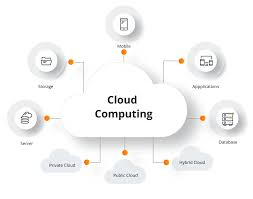
\includegraphics [scale=0.9] {figures/cloud}
	\caption{Architecture of cloud computing}
	\label{fig01}	
\end{figure} 
The data are shown in Table \ref{tab01}
% Please add the following required packages to your document preamble:
% \usepackage[table,xcdraw]{xcolor}
% Beamer presentation requires \usepackage{colortbl} instead of \usepackage[table,xcdraw]{xcolor}
\begin{table}[h]
	\centering
	\begin{tabular}{|c|c|c|}
		\hline
		\rowcolor[HTML]{67FD9A} 
		One & Two   & three \\ \hline
		\rowcolor[HTML]{EFEFEF} 
		1   & 2     & 3     \\ \hline
		One & Thrre & Four  \\ \hline
	\end{tabular}
	\caption{Data for Cloud}
	\label{tab01}
\end{table}



